\documentclass{amsart}

\synctex=1

\usepackage{amsmath,amsthm}
\usepackage{todonotes}
\usepackage{natbib}
\usepackage[notref,notcite]{showkeys}
\usepackage{enumerate}
\usepackage{url}
\usepackage[colorlinks=true]{hyperref}
\usepackage{graphicx}

\newtheorem{lemma}{Lemma}
\newtheorem{question}[lemma]{Question}
\newtheorem{proposition}[lemma]{Proposition}
\newtheorem{corollary}[lemma]{Corollary}
\newtheorem{theorem}[lemma]{Theorem}

\newcommand{\dts}{\mathrm{DtT}}
\newcommand{\nni}{\mathrm{NNI}}
\newcommand{\rnni}{\mathrm{rNNI}}
\newcommand{\mdts}{\mathrm{mDtT}}
\newcommand{\MH}{\mathrm{MH}}
\newcommand{\ric}{\operatorname{ric}}
\newcommand{\rt}{\mathrm{rt}}
\newcommand{\tp}{\mathrm{tp}}

\renewcommand{\O}{\mathcal{O}}

\begin{document}

\section{Introduction}
%%%%%%%%%%%%%%%%%%%%%%%%%%%%%%%%%%%%%%%%%%%%%%%%%%%%%%%%%%%%%%%%%%%%%%%%%%%%%%%%

In this paper we study Ricci-Ollivier curvature of Markov chains over phylogenetic trees \cite{Ollivier2009-cj}.
We formalize different spaces of phylogenetic trees as graphs, where the adjacency
relation is given by a tree move. Those graphs can be also seen as metric
spaces where the distance between two points is given by the length of a
shortest path connecting them. All graphs we are considering in this paper are
connected, so thus defined distance is indeed a metric.

A Markov chain (often a random walk in our case) is defined on a graph by its
proposal mechanism, which is a functional $m$ that maps vertices of the graph to
the set of measures on this graph. In other words, for every vertex $v$,
$m_v(w)$ is the probability of moving from $v$ to $w$ in one step.
Given a graph with vertices ${u, v, \ldots}$, a \emph{coupling} $\{p_{u,v}\}$ between two measures $\mu$ and $\nu$ is a probability measure on $V(G) \times V(G)$ that is $\mu$ after marginalizing over the second component, and $\nu$ after marginalizing over the first.

We consider a number of Markov chains that arise in phylogenetic Bayesian inference and investigate the curvature of those chains with the eventual goal of the efficiency properties of the corresponding inference methods.

\section{Discrete time-tree space and its variants}
%%%%%%%%%%%%%%%%%%%%%%%%%%%%%%%%%%%%%%%%%%%%%%%%%%%%%%%%%%%%%%%%%%%%%%%%%%%%%%%%

In this section we introduce a discrete analogue of the space of time-trees and establish several graph-theoretic properties of this space, which will be used to study the curvature of certain random walks on the space.
We also consider three other tree spaces, which have similar properties as time-trees, as we shall see.

It is generally assumed that a time-tree is an ultrametric phylogenetic tree, that is, a tree with all leaves sampled at present.
All results in this paper can be derived for the discrete counterpart of such space.
However, there is no need to restrict ourselves by the ultrametricity property, as the results can be obtained in the more general setting of rooted phylogenetic trees with branch lengths.
Moreover, many biological application explicitly require the restriction imposed by ultrmetricity to be dropped~\cite{}.
Hence, by a time-tree in this paper we mean a rooted phylogenetic tree.

\todo[inline]{Should we add some other trees? Ultrametric trees? Ranked NNI as Chris initially understood it?}

In short, the {\em discrete time-tree space,} or $\dts$ space, is the $\tau$-space defined in~\cite{Gavryushkin2014-bw}, where the intercoalescent intervals are allowed to take only two length values, $1$ and $2$.
In other words, to define a tree in $\dts$, we first fix a ranked tree topology with all nodes being of different ranks and then assign a number from $\{1,2\}$ to every intercoalescent interval.
Intuitively, we have only two options for the length of an intercoalescent interval, which can be thought of as short and long.
We shall describe the numbers assigned to the intercoalescent intervals as to the {\em lengths} of those intervals.

We now go on to defining the adjacency relation of the graph $\dts$, the set of vertices of which consists of $\dts$ trees.
In short, two trees in $\dts$ are adjacent if the $\tau$-geodesic, defined in~\cite{Gavryushkin2014-bw}, crosses precisely one face of co-dimension $1$.
To make this paper self-contained, we provide a complete definition below, for which the following notions are needed.
Let $T$ be a rooted phylogenetic tree with branch lengths such that the ranked topology of $T$ inherited from its branch lengths does not have two nodes (including taxa) of the same rank.
We denote this ranked topology by $\rt(T)$ and assume that all nodes of the tree (including taxa) are assigned ranks $0,1,\ldots$
The node of rank $0$ is seen as being at the present, so the root has the highest rank and is the oldest node of the tree.
An {\em intercoalescent interval} of $T$ is an interval between any two nodes of consecutive ranks.
Intercoalescent intervals of a tree on $6$ taxa are depicted on Figure~\ref{T5.pdf}.
By $\ell_T(I)$ we denote the length of the intercoalescent interval $I$ in tree $T$.
We say that two trees $T$ and $R$ {\em have the same ranked topology} and write $\rt(T) = \rt(R)$ if the tree topologies are isomorphic as directed graphs and the isomorphism preserves ranks of the nodes.
In the same way we write $\tp(T) = \tp(R)$ when trees $T$ and $R$ have the same rooted tree topology (that is, ranks are ignored).

\begin{figure}
\centering
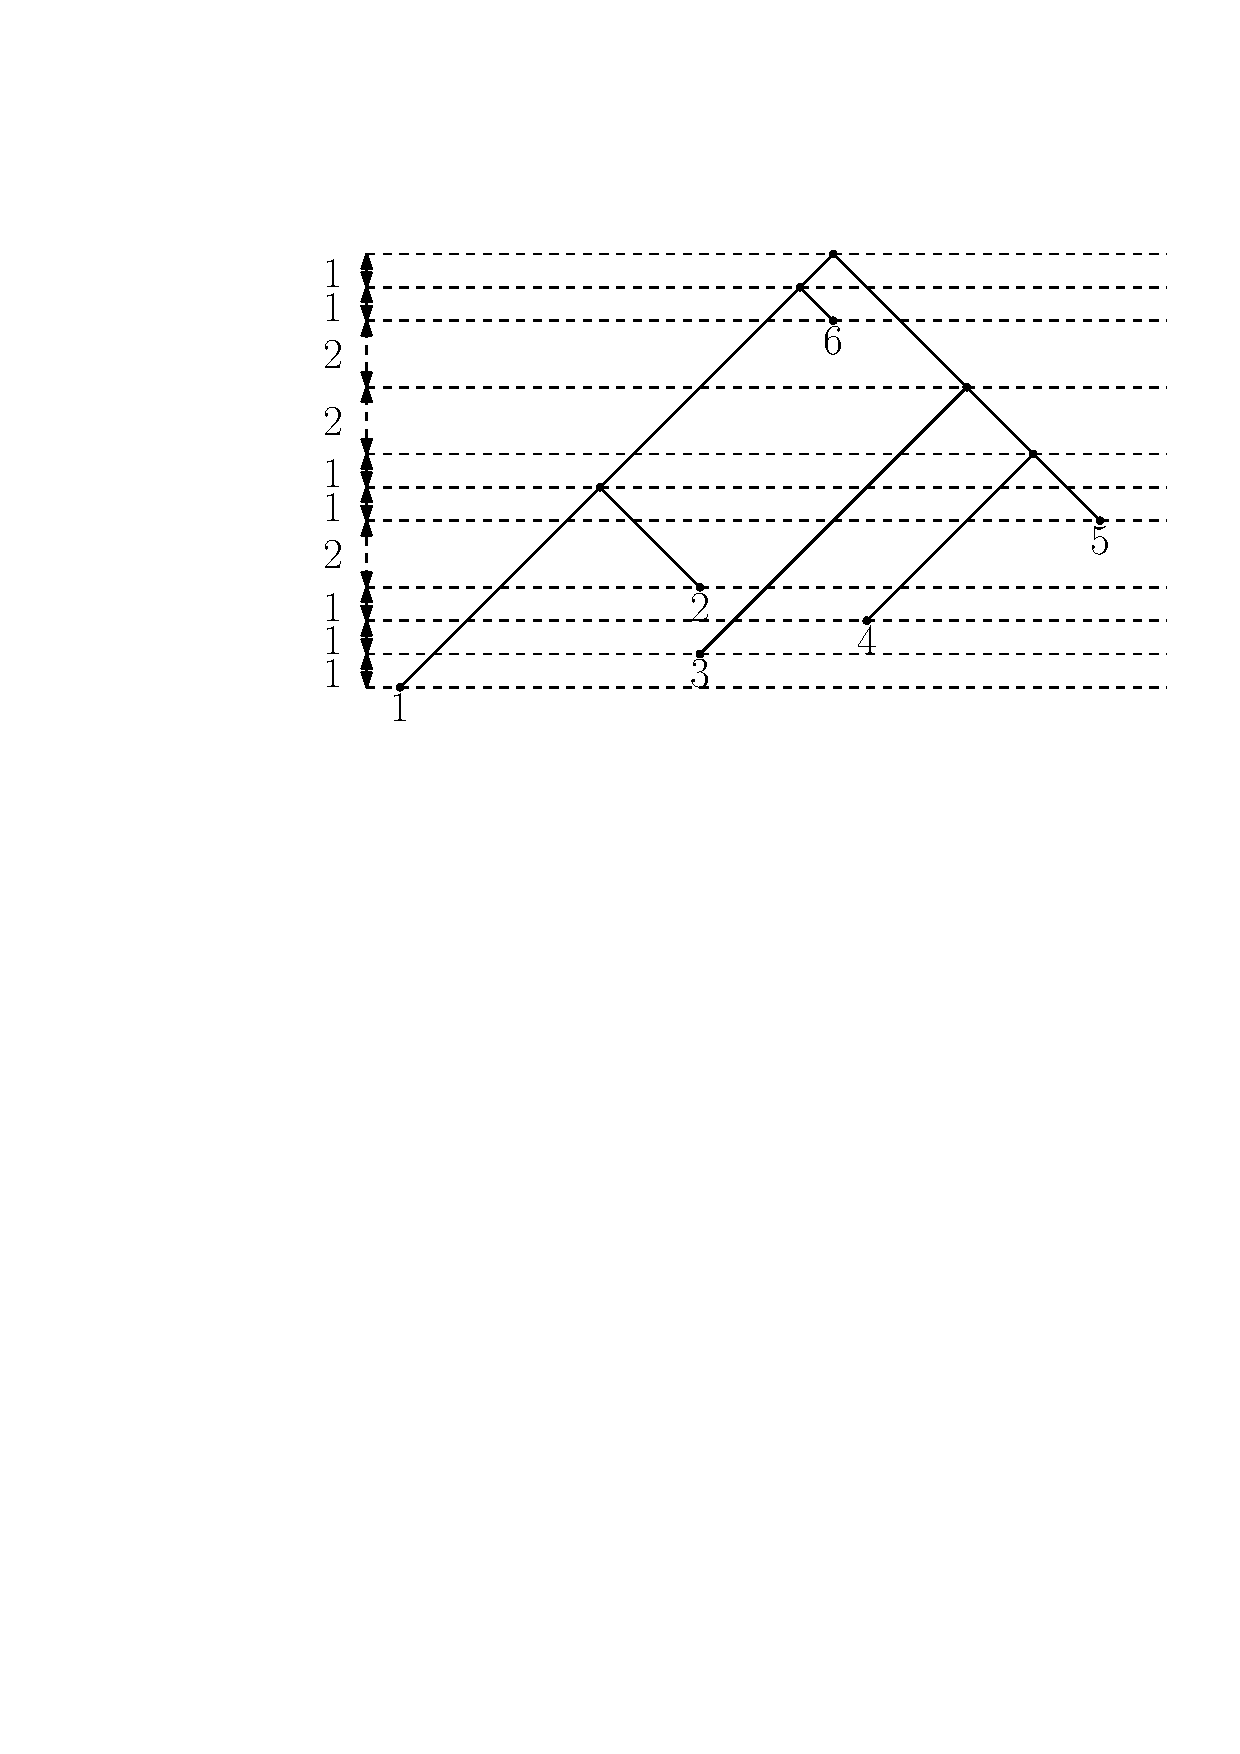
\includegraphics[width=0.7\textwidth]{T5.pdf}
\caption{Intercoalescent intervals with their lengths of a tree from $\dts$ on $6$ taxa.}
\label{T5.pdf}
\end{figure}

We say that two trees $T$ and $R$ are {\em NNI neighbours} if $\rt(T) \ne \rt(R)$ and tree $R$ is obtained from tree $T$ by sending the length of an intercoalescent interval between an internal node and its parent in $T$ down to zero and resolving the multifurcation in one of the two possible ways.
We note that this definition implies the existence of such an interval in $T$, that is, the existence of an internal node $a$ the parent of which is the immediate successor of $a$ in $\rt(T)$.
In particular, the parent of $D$ in tree $T$ on Figure~\ref{dts_neighbours.pdf} gives an example of such a node $a$.
Note also that the parent of $C$ in $T$ denoted by $b$ on Figure~\ref{dts_neighbours.pdf} does not satisfy this property, that is, the parent of $b$ is not its immediate successor in $\rt(T)$.
Hence, the tree obtained from $T$ by cutting the edge adjacent to $C$ and regrafting it to the edge between the aunt of $b$ and the root does not give an NNI neighbour of $T$ in this sense.
Note that the definition of NNI neighbours implies $\ell_T(J) = \ell_R(J)$ for each interval $J \ne I$, and the ranks of all nodes present in both $T$ and $R$ coincide.
If trees $T$ and $R$ are NNI neighbours and tree $R$ is obtained by suppressing an interval $I$ in $T$ then we say that the {\em NNI move is performed on interval $I$}.

Two trees $T$ and $R$ from $\dts$ are adjacent if and only if precisely one of the following conditions is satisfied.
\begin{enumerate}[(1)]
\item $\rt(T) = \rt(R)$ and there exists a unique intercoalescent interval $I$ such that $|\ell_T(I) - \ell_R(I)| = 1$.
\item $\tp(T) = \tp(R)$, there exists a unique pair of nodes $a,b$ with consecutive ranks in $\rt(T)$ such that the ranks of $a$ and $b$ are swapped in $R$, the intercoalescent interval $I$ between $a$ and $b$ satisfies $\ell_T(I) = \ell_R(I) = 1$, and $\ell_T(J) = \ell_R(J)$ for all other intervals $J \ne I$.
\item $T$ and $R$ are NNI neighbours and $\ell_T(I) = \ell_R(I) = 1$ where the NNI move is performed on interval $I$.
\end{enumerate}

In other words, by going from one tree to an adjacent tree in $\dts$ graph we can either change the length of one intercoalescent interval by one unit or we can send the length of an intercoalescent interval of minimal length down to zero and then resolve the multifurcation to either of the two possible topologies (one possible topology if there is no multifurcation) and assign the minimal length to the new interval.
See Figure~\ref{dts_neighbours.pdf} for an example of a pair of trees $T,R$ at $\dts$ distance $3$, where one has to apply all of the three possible cases from the definition above to obtain a path from $T$ to $R$ in $\dts$.

\begin{figure}
\centering
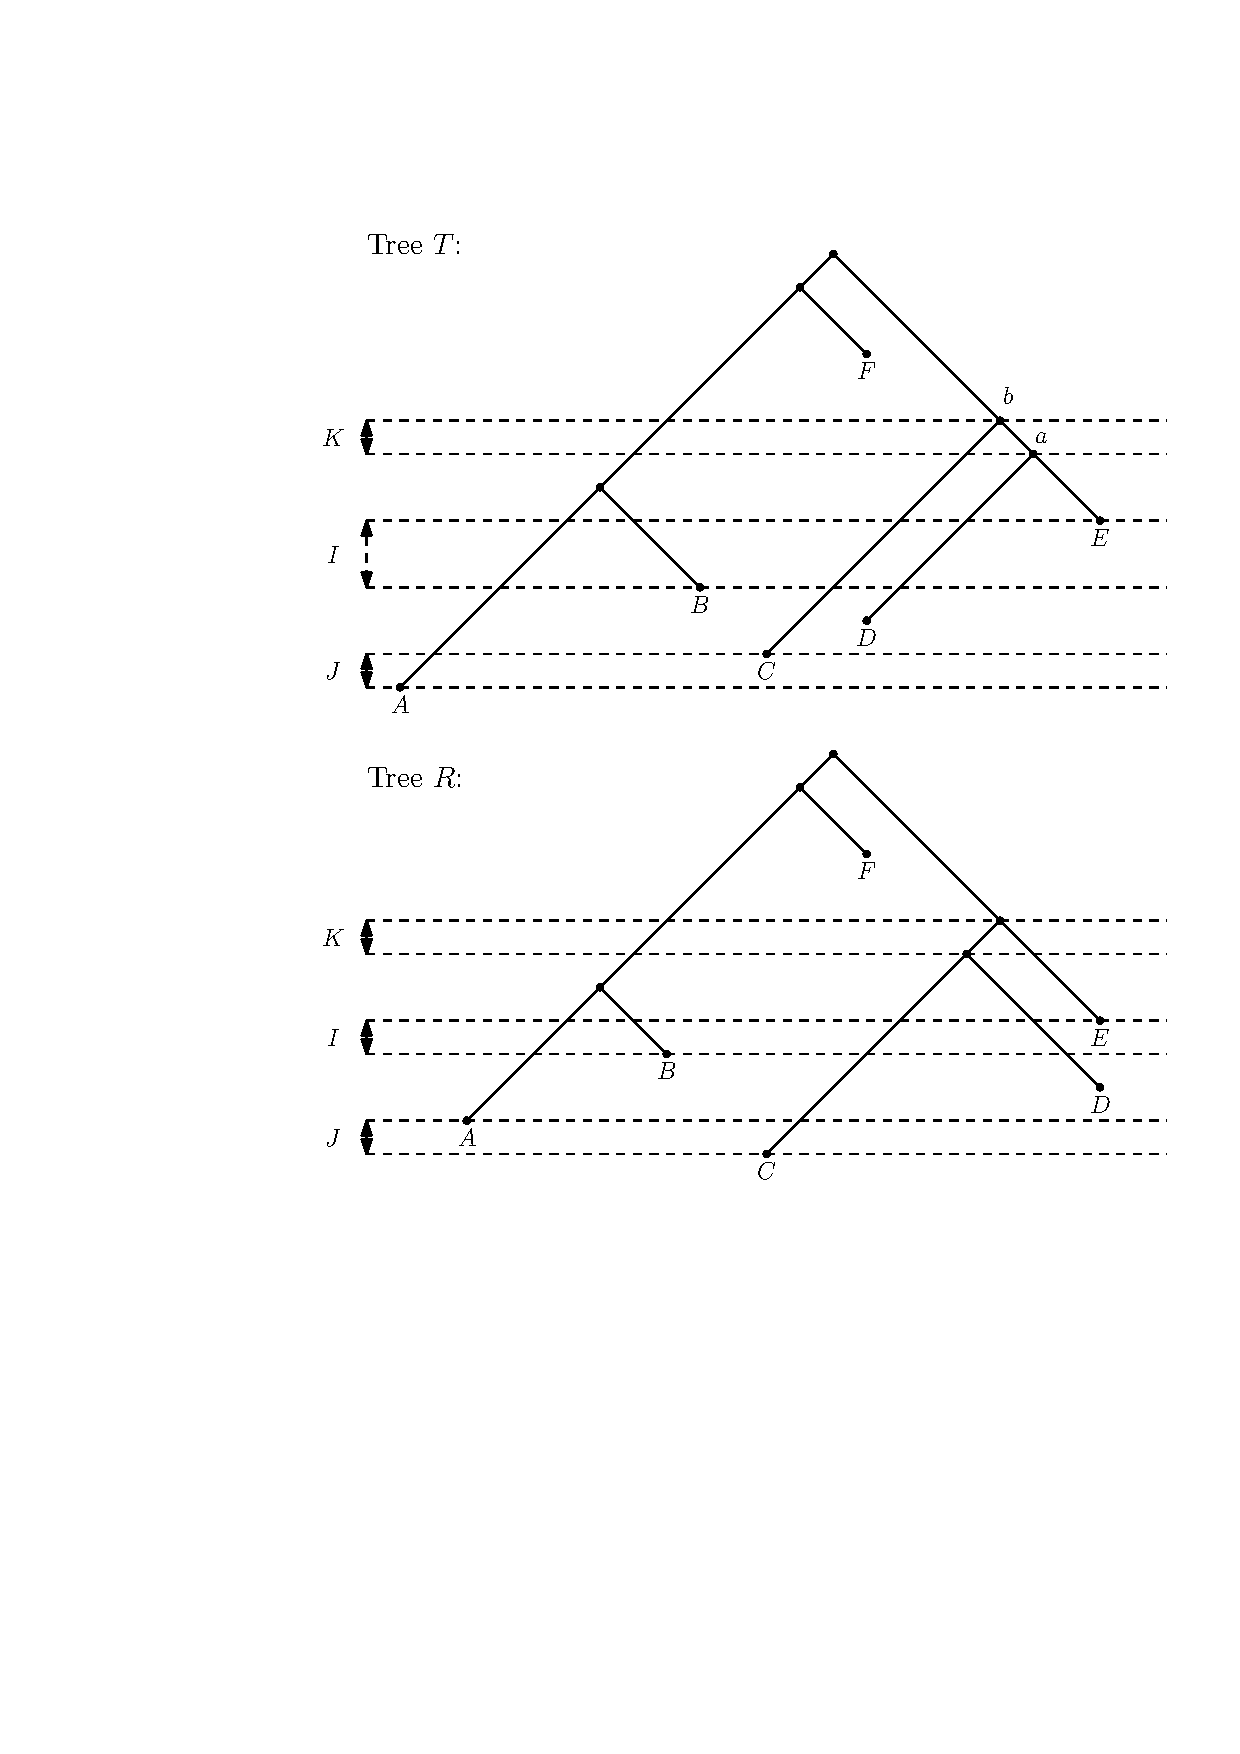
\includegraphics[width=0.7\textwidth]{dts_neighbours.pdf}
\caption{Trees $T$ and $R$ are at $\dts$ distance $3$.
To move from $T$ to $R$ in $\dts$, one must decrease the length of interval $I$, swap the ranks of nodes $A$ and $C$ bounding the interval $J$, and perform an NNI move on interval $K$, resolving nodes $C$ and $D$.}
\label{dts_neighbours.pdf}
\end{figure}

Thus we have defined a graph, which we denote by $\dts$.
Since a graph can also be seen as a metric space where the distance is given by the length of a shortest path, we will refer to $\dts$ as both.

One might suggest that geometrically and graph-theoretically $\dts$ is similar to NNI space on (rooted) tree topologies, to ranked NNI space, and to $\dts$ space with an arbitrary (but finite) number of intercoalescent interval lengths.
That is so indeed.
As we shall see, the results and proofs in this paper can be straightforwardly adapted to the spaces mentioned.
Furthermore, as the NNI space of unrooted tree topologies with $n-1$ leaves is isomorphic (as a graph) to the NNI space of rooted tree topologies with $n$ leaves, all our results immediately imply their counterparts in unrooted NNI space.
We omit from the text the exact formulations for unrooted trees, as they can be obtained in the obvious way.
We will provide complete proofs for $\dts$ space and draw the corresponding results for the other three treespaces simultaneously.

We denote NNI space on rooted tree topologies by $\nni$.
The $\dts$ space with only short branches is denoted by $\rnni$ and called {\em ranked NNI} space.
The space of $\dts$ trees with $m$ branch lengths is denoted by $\mdts$.
All of these can be considered as either a graph or a metric space, and we will refer to them as both.
By $n$ we denote the number of taxa and assume $n \geq 3$ throughout the paper.

\begin{lemma}\label{neighBound}
Let $T$ be a tree on $n$ leaves. 
Then
\[2(n-1) \leq \deg(T) \leq 5n-6\] in $\dts$ and $\mdts$ space,
\[\deg(T) = 2(n-2)\] in $\nni$ space, and
\[n-1\leq \deg(T) \leq3n-4\] in $\rnni$ space.
\end{lemma}

\proof
The lower bound in $\dts$ and $\mdts$ spaces is attained by any tree with all intercoalescent intervals being long.
In this case, $\deg(T)$ is simply the number of intercoalescent intervals, since every intercoalescent interval adds $1$ to the total degree of the tree.
Other trees have the same or more possible intercoalescent interval changes, showing that this is a lower bound.
The upper bound is attained by a caterpillar tree with all intervals short and no coalescent event being younger than a taxon.
In this case, $\deg(T)$ is $2(n-1)$, the number of intervals---comes from the interval length changes, plus $2(n-2)$, the maximal possible number of NNI neighbours, plus $n$, the number of rank changes between taxa.
In total, $2(n-1) + 2(n-2) + n = 5n-6$.
Note that this is an upper bound indeed, as each of the $2(n-2)$ intervals excluding the most recent can contribute either a rank change or $2$ NNI moves.
Clearly, the tree described maximises the number of intervals that contribute $2$ NNI moves and enables the rest of intervals to contribute a rank change.

Note also that no other tree class attains the upper bound in $\dts$ space.\todo{This is actually the only property mentioned so far that distinguish DtT and mDtT.
This should be taken care of when we decide what spaces we keep.}

Since every NNI move results in two neighbours, the equality $\deg(T) = 2(n-2)$ follows.
Indeed, it is not hard to see that the set of NNI moves that only consider moving a subtree to its aunt captures the full set of NNI neighbors with no duplicates.
The neighborhood size then follows because the root and its two children have no aunt.

The lower bound in $\rnni$ space is attained by the caterpillar-tree where taxa get ranks $1, 2, 4, 6, \ldots$ and internal nodes get ranks $3, 5, 7, \ldots$
In other words, the coalescent events alternate with the taxa in the ranked topology of the tree so that if we parse the tree from the present to the past, we meet the nodes in the following order: taxon, taxon, coalescence, taxon, coalescence, taxon, coalescence$\ldots$
%\todo{EM: A little more detail, please? The nodes are numbered so far, not the intervals\\ 
%AG: fixed.\\
%EM: OK, thanks, though in the next sentence you still do talk about even and odd {\em intervals}.\\
%AG: fixed.}
In this case, intervals bounded by a taxon from below add nothing to the degree of the tree and intervals bounded from below by an internal node add one each, hence $n-1$ in total.
The upper bound is obtained in the same way as for $\dts$ and $\mdts$ spaces.
\endproof

We will need the following obvious corollaries for our analysis of curvature.

\begin{corollary}\label{degreeBounds}
The following are satisfied in both $\dts$ and $\mdts$ spaces for any trees $T$ and $R$.
\begin{enumerate}[(1)]
\item $deg(T)-deg(R) \leq 3(n-1)$.
\item $\dfrac25 \leq \dfrac{\deg(T)}{deg(R)} \leq \dfrac52$, and the equality is attained for both bounds and all $n$.
\end{enumerate}
\end{corollary}

\proof
Follows from Lemma~\ref{neighBound}.
\endproof

For $\nni$ space, Lemma~\ref{neighBound} implies that $deg(T)-deg(R) = 0$ and $\frac{\deg(T)}{deg(R)} = 1$.

\begin{corollary}\label{degreeBoundsNNI}
The following are satisfied in $\rnni$ space.
\begin{enumerate}[(1)]
\item $deg(T)-deg(R) \leq 2(n-2)$.
\item $\dfrac13 \leq \dfrac{\deg(T)}{deg(R)} \leq 3$, and the equality is attained for both bounds and all $n$.
\end{enumerate}
\end{corollary}

\proof
Follows from Lemma~\ref{neighBound}.
\endproof

Let $N(T)$ be the set of trees at distance one from $T$, that is, the set of trees adjacent to $T$ in the corresponding graph.
The following lemma describes how many trees the tree neighbourhoods can have in common.

\begin{lemma}\label{intersecNeighb}
The following is true for all four spaces $\nni$, $\rnni$, $\dts$, and $\mdts$.
If $d(T,R) = 1$ then $|N(T)\cap N(R)|\in\{0,1\}$.
\end{lemma}

\proof
Suppose $T$ and $R$ are neighbours.
If the trees differ by a single branch length or rank change then the fact that NNI moves only apply to short branches implies that any shared neighbour $S$ would have to match the length or rank of one of the trees. As $S$ must differ from both trees, they do not have a neighbour in common.
If $T$ and $R$ are NNI-neighbours, there is precisely one tree which is a neighbour of both $T$ and $R$, namely the third tree that can be obtained by resolving the interval that connects $T$ and $R$.
%\todo[inline]{EM: Clarify please?} CW&AG: Fixed.
\endproof

The following general lemma is true for all graphs, particularly, for those we consider in this paper.
By {\em distance-one random walk}, we mean a random walk $(m_x)_{x \in X}$ satisfying $m_x(y) = 0$ for all $x$ and $y$ such that $d(x,y) > 1$.

\begin{lemma}\label{curvBoundGeneral}
Let $(M,d)$ be a finite metric space and $x,y$ a pair of points from $M$. If
$(m_x)_{x \in M}$ is a distance-one random walk on $M$, then the curvature
$\kappa$ of the random walk satisfies the following boundary conditions.
\[
\dfrac{-2}{d(x,y)} \leq \kappa(x,y) \leq \dfrac{2}{d(x,y)}.
\]
\end{lemma}

\proof
Let $x$, $y$, $u$, and $v$ be arbitrary points from $M$ such that both $m_x(u)$
and $m_y(v)$ are positive. Since $m$ is a distance-one random walk,
$d(u,v) \leq d(x,y) + 2$. Hence for any coupling $\{p_{u,v}\}$,
\[
W(m_x,m_y) \leq \sum p_{u,v} d(u,v) \leq (d(x,y)+2)\sum p_{u,v} = d(x,y) + 2,
\]
where the sum is taken over a correspondence between the set of $u \in N(x)$ and
$v \in N(y)$. So, $\kappa(x,y) \geq - 2/d(x,y)$. The lower bound follows
similarly from $d(u,v) \geq d(x,y) - 2$.
\endproof

Note that this lemma can be generalised to {\em distance-$d$} random walks,
which are those satisfying $m_x(y) = 0$ for all $x$ and $y$ such that
$d(x,y) > d$. In this case, the curvature bounds are
\[
-\dfrac{2d}{d(x,y)} \leq \kappa(x,y) \leq \dfrac{2d}{d(x,y)}.
\]
For one needs to notice that in the notations of the lemma,
$d(u,v) \leq d(x,y) + 2d$.

As we will see in the next few lemmas, these bounds can be improved for certain random walks on the graphs under consideration.

\begin{lemma}\label{uniformUpper}
Let $T$ and $R$ be adjacent trees.
Then the curvature of the spaces with uniform random walk satisfy
\[
\kappa(T,R) \leq \dfrac{1}{2(n-1)}
\]
for $\dts$ and $\mdts$ spaces,
\[
\kappa(T,R) \leq \dfrac{1}{2(n-2)}
\]
for $\nni$ space, and
\[
\kappa(T,R) \leq \dfrac{1}{n-1}
\]
for $\rnni$ space.

The bounds are tight.
\end{lemma}

\proof
To maximise the curvature $\kappa(T,R)$, we have to minimise $W(m_T,m_R)$.
The latter is minimised when the probability mass on trees of distance zero or one away from $R$ is maximized.
\todo{TODO: clarify this. We should be talking about where the mass is in the coupling.}
Since $d(T,R) = 1$, it follows from Lemma~\ref{intersecNeighb} that this probability mass is positive only when $|N(T) \cap N(R)| = 1$. 
It follows from Lemma~\ref{neighBound} that the maximal mass we can allocate under a uniform random walk to the tree in $N(T) \cap N(R)$ is $\frac{1}{2(n-1)}$ in $\dts$ and $\mdts$ spaces, $\frac{1}{2(n-2)}$ in $\nni$ space, and $\frac{1}{n-1}$ in $\rnni$ space.
The lemma follows.
\endproof

%\todo[inline]{You use "corollary" in a different sense than I've seen before. I have only seen it used to mean "follows directly from the theorem/lemma but you seem to use it as "follows from a similar line of argument."} AG: fixed.

This lemma and corollary provide tighter upper bounds for the curvature than Lemma~\ref{curvBoundGeneral} for all $n$.

It is easy to generalise the lemma to the uniform $p$-lazy random walk.
Indeed, by looking at the proof of the lemma, one can notice that the curvature between adjacent trees $T$ and $R$ under a uniform $p$-lazy random walk satisfies
\[
\kappa(T,R) \leq \frac{p}{2(n-1)}
\]
in $\dts$ and $\mdts$ spaces,
\[
\kappa(T,R) \leq \frac{p}{2(n-2)}
\]
in $\nni$ space, and
\[
\kappa(T,R) \leq \frac{p}{n-1}
\]
in $\rnni$ space.

%\todo{This can get confusing fast. Please see \url{https://matsengrp.slack.com/files/matsen/F04J79F5A/pasted_image_at_2015_04_27_07_08_am.png} for definition of asymptotic ricci curvature. I suggest using $\operatorname{ric}$ for this quantity.} AG: fixed.

We follow Loisel and Romon~\cite{Loisel2014-gu} and define {\em asymptotic Ricci-Ollivier curvature} $\ric$ of a metric space with uniform $p$-lazy random walk by 
\[
\ric(x,y) = \lim_{p\to0} \frac{\kappa(x,y)}{p}
\]

In this case the asymptotic curvature between adjacent trees in $\dts$ and $\mdts$ with uniform $p$-lazy random walk is bounded from above by
\[
\frac{1}{2(n-1)}
\]

Following Loisel and Romon~\cite{Loisel2014-gu}, we will refer to non-asymptotic curvature as {\em coarse curvature} \todo{Should this go into the intro? AG tends to leave it here because otherwise the reader will have to go back at this point to refresh the def's.} to distinguish between the two alternative notions of curvature.


Thus, the upper bound of asymptotic curvature of $\nni$, $\rnni$, $\dts$, and $\mdts$ spaces coincides with the coarse curvatures of the spaces.

We continue with lower bounds on curvature of spaces with uniform lazy random walks.

\begin{lemma}\label{uniformLower}
Let $T$ and $R$ be adjacent trees.
Then both the asymptotic curvature of the space with $p$-lazy uniform random walk and the curvature of the space with uniform random walk are at least 
\begin{enumerate}[(i)]
\item $-\dfrac{4}{n-1}$ in $\dts$ and $\mdts$ spaces,
\item $-\dfrac{4}{n-2}$ in $\nni$ space,
\item $-\dfrac{8}{n-1}$ in $\rnni$ space. 
\end{enumerate}

The bounds are tight.
\end{lemma}

\proof
Let $T$ and $R$ be two adjacent trees. To minimise the curvature, we have
to maximise $W(m_T, m_R)$ across $T$ and $R$. The latter is maximised when the probability mass
on trees $E\in N(T)$ such that $d(E, N(R)) > d(T, R)$, is
maximised\footnote{If $x$ is a point of a metric space $(M,d)$ and
$S \subseteq M$ then by $d(x,S)$ we denote $\inf\limits_{s \in S} d(x,s)$.}.
Since $d(T, R) = 1$, the maximum possible number of such trees $E$ is
\todo{Explain this. EM skipped pending explanation.}
$8$. To make $W(m_T,m_R)$ being as large as possible, we have to assume
$d(S, N(R)) = 1$ for the rest of the trees $S$ from $N(T)$.
Hence for the uniform random walk we have:
\[
W(m_T,m_R)\leq 8 \cdot 2 \cdot \frac{1}{|N(T)|} +
(|N(T)| - 8) \cdot \frac{1}{N(T)} = 1 + \dfrac{8}{|N(T)|}.
\]
Hence, $\kappa(T,R) = 1 - W(m_T,m_R) \geq - \dfrac{8}{|N(T)|}$.

A similar reasoning applies for the $p$-lazy random walk:
\[
W(m_T,m_R)\leq 8 \cdot 2 \cdot \frac{p}{|N(T)|} +
(|N(T)| - 7) \cdot \frac{p}{|N(T)|} + (1-p) - \frac{p}{|N(T)|} =
\]
$1 + \dfrac{8p}{|N(T)|}$. Hence,
$\ric(T,R) = \lim\limits_{p\to0}\left(1 - W(m_T,m_R)\right) \geq - \dfrac{8}{|N(T)|}$.

It remains to note that Lemma~\ref{neighBound} gives us an estimate $|N(T)| \geq 2(n-1)$ in $\dts$ and $\mdts$, $|N(T)| \geq 2(n-2)$ in $\nni$, and $|N(T)| \geq n-1$ in $\rnni$ space.
The lemma follows.
\endproof

\begin{corollary}\label{flatInLimDTS}
Let $(T_n,R_n)_{n\in\omega}$ be a sequence of pairs of trees such that
$d(T_n,R_n) = 1$ in $\nni$, $\rnni$, $\dts$, or $\mdts$ space.
Then $\lim\limits_{n \to \infty}\kappa(T_n,R_n) = \lim\limits_{n \to \infty}\ric(T_n,R_n) = 0$.
\end{corollary}

\proof
Follows from Lemma~\ref{uniformUpper} and Lemma~\ref{uniformLower}.
\endproof

As we have just proved, the corollary above holds true in $\nni$, $\rnni$, $\dts$, and $\mdts$ spaces.
This corollary is also true in the SPR space of rooted trees~\cite{Whidden2015-es}.
Actually, this property can be derived from the following general statement for all spaces mentioned, as well as for many others.

\begin{proposition}\label{flatInLimGen}
Let $(M_n,d_n)_{n \in \omega}$ be a sequence of finite metric spaces and
$(x_n, y_n)$ a sequence of adjacent vertices from $M_n$,
that is $d_n(x_n,y_n) = 1$, such that
\begin{enumerate}[(1)]
\item\label{intersec} $\big|N(x_n) \cap N(y_n)\big| = o(|N(x_n)|)$
\item\label{difference} $\big||N(x_n)| - |N(y_n)|\big| = o(|N(x_n)|)$
\item\label{dist2} $\big|\{(x,y) \mid
	x \in N(x_n),~ y \in N(y_n),~ d(x, y) \geq 2\}\big| = o(|N(x_n)|)$
\end{enumerate}

Then $\lim\limits_{n \to \infty} \kappa(x_n, y_n) = 0$.
\end{proposition}

\proof
Consider an arbitrary $n$ and the pair of points $x_n,y_n$.
Set $I_0 = N(x_n) \cap N(y_n)$, denote by $I_1$ the set of points
$z$ such that the probability mass is moved from $z$ at distance one under the
optimum coupling for $W(m_{x_n},m_{y_n})$, by $I_2$ the set of points $z$ such that
the probability mass is moved from $z$ a distance $\geq 2$ under the optimum
scenario for $W(m_x,m_y)$. Then
\[
W(m_{x_n},m_{y_n}) = \sum_{I_0} d_i x_i p_{x_i} + \sum_{I_1} d_i x_i p_{x_i} +
\sum_{I_2} d_i x_i p_{x_i}.
\]
%\todo{I'm not sure why \ref{intersec}) is needed here.} AG: the typo fixed.
It follows from~(\ref{intersec}) and~(\ref{dist2}) that the first and the last sums
are $\O(1)$ when $n\to\infty$. This together with property~(\ref{difference})
implies that the middle sum tends to $1$ when $n\to\infty$ because the number of
points $z$ such that the probability mass has to travel at distance one under an
optimum scenario, divided by $|N(x_n)|$, tends to $1$ when $n\to\infty$.
\endproof

We note that in both Corollary~\ref{flatInLimDTS} and Proposition~\ref{flatInLimGen}, the assumption of being at distance one can be relaxed by that of being at a distance uniformly bounded by a slowly growing function.
But since the primary focus of this paper is on the spaces under consideration, we will not \todo{Should we?} include the statement in general terms of metric spaces.
However, we prove below (Theorem~\ref{zero-in-the-limit}) a much stronger property of the spaces, namely, that the curvature tends to zero when the tree size tends to infinity does not matter what distance between the trees is.

We first bound the number of neighbors of a tree $x$ in $\dts$-space that are closer than $x$ to a given tree $y$.
We show that the maximum fraction of neighbors that tend closer to $y$ grows linearly with respect to $d(x,y)$.
These subsets of neighbors are the force pushing towards positive curvature, so this will allow us to bound the maximum curvature with respect to distance.
%\todo{I put this here for now, but it will have to go earlier.} AG: fixed.

\begin{theorem}
\label{max_good_neighbors}
Let $x$ and $y$ be two trees.
Then the number of trees $u \in N(x)$ such that $d(u, y) \le d(x, y)$ is at most 
\begin{enumerate}[(i)]
\item $2d(x,y)$ in $\nni$ space,
\item $3d(x,y)$ in $\rnni$ space,
\item $4d(x,y)$ in $\dts$ space,
\todo{How is this consistent with the $8$ in Lemma~\ref{uniformLower}?}
\item $5d(x,y)$ in $\mdts$ space.
\end{enumerate}
\end{theorem}

\begin{proof}
We first prove the statement for $\dts$ space.

Let $U$ be the set of neighbors $u$ of $x$ such that $d(u,y) \le d(x,y)$, as stated in the theorem.
We partition $U$ into three sets of trees---$I$, $R$, and $L$---obtained from $x$ by a single NNI move, rank change, or length change, respectively.
We then prove the theorem by bounding the size of each partition by $2d(x,y)$, $d(x,y)$, and $d(x,y)$, respectively.

We first consider some basic properties of minimal length paths between $x$ and $y$.
Observe that at most $d(x,y)$ bipartitions differ between $x$ and $y$, as each NNI operation replaces one bipartition with another (and rank and length changes do not modify bipartitions).
Now, observe that no minimal length path from $x$ to $y$ will replace a bipartition that is common to $x$ and $y$, as any path including such a replacement can be made shorter by removing the replacement move (and subsequent moves that reintroduce the bipartition).

We are now ready to bound the sizes of each partition $I$, $R$, and $L$.
First, consider the subset $I$ of closer neighbors obtained via NNI moves.
By our observations above, $|I|$ is bounded by the number of NNI operations that modify one of the at most $d(x,y)$ bipartitions of $x$ that are not a bipartition of $y$.
There are two neighbors of $x$ that lack any given bipartition (obtained by moving either the left or right subtree located below the bipartition).
Therefore, $|I| \le 2d(x,y)$.

Second, consider the subset $R$ of closer neighbors obtained via rank change moves.
These operate either on one of $x$'s unique bipartitions or a bipartition common to $x$ and $y$ that differs in rank.
As observed above, the number of unique bipartitions is bounded by the maximum number of NNI moves on any minimal $x$ to $y$ path.
Any such path must fix the ranks of each common edge.
In other words, if $r_1$ is the number of trees in $U$ which are obtained from $x$ by a rank move corresponding to a common edge and $r_2$ is the number of trees in $U$ which are obtained from $x$ by a rank move corresponding to a unique edge of $x$, then $r_1 + r_2 \leq d(x,y)$, because the $r_1$ moves have to be done along every shortest path from $x$ to $y$.
Thus, the total size of $R$ is bounded by $d(x,y)$.

The bound of $d(x,y)$ on the number of length changes that can be applied to move $x$ closer to $y$ follows similarly.
Therefore, there are at most $|I| + |R| + |L| \le 2d(x,y) + d(x,y) + d(x,y) = 4d(x,y)$ trees $u \in N(x)$ such that $d(u, y) \le d(x, y)$.

The statement for the other three spaces follows similarly: for $\nni$ we need to count only for trees from $I$, for $\rnni$ we need to count only for trees from $I$ and $R$, for $\mdts$ we will have to add $2d(x,y)$ instead of $d(x,y)$ for $L$.
\end{proof}

%\todo[inline]{I suggest folding all of this into the above theorem, along with a statement in the proof saying that the extra statements follow similarly.}
%Note that this implies the following corollaries for $\nni$, $\rnni$ and $\mdts$ spaces. AG: fixed.

We now use Theorem~\ref{max_good_neighbors} to prove the following.
\todo[inline]{v This must be true for $p$-lazy walk as well.}

\begin{theorem}\label{zero-in-the-limit}
Let $(T_n,R_n)_{n\in\omega}$ be a sequence of pairs of $\dts$-trees on $n$ taxa.
Then $\lim\limits_{n \to \infty}\kappa(T_n,R_n) = 0$ for the uniform random walk.
\end{theorem}

\proof
One of the main properties of Ollivier-Ricci curvature\footnote{Note that we are considering only finite metric spaces.
However, the result holds true for all metric spaces.}
is that the curvature is a local property~\cite{Ollivier2009-cj}, that is, for all distinct $u$ and $v$,
\[
\inf\{\kappa(x,y)\mid d(x,y) = 1\} \leq \kappa(u,v).
\]
Hence, it follows from Lemma~\ref{uniformLower} that $\kappa(T_n,R_n) \geq -\dfrac{4}{n-1}$ for all $n$.
To finish the proof, we need to bound the sequence $\kappa(T_n,R_n)$ from above by another sequence which tends to zero.

Let us fix an $n$ and let $U$ be the set of trees $E \in N(T)$ such that $d_\dts(E,R_n) \leq d_\dts(T_n,R_n)$ as in Theorem~\ref{max_good_neighbors}, and $B$ be the rest of trees $N(T_n)\setminus U$ from $N(T_n)$.
Let's denote $d_\dts(T_n,R_n)$ by $d$. Then
\[
W(m_{T_n},m_{R_n}) = \sum_{i\in U} p_i d_i + \sum_{j\in B} p_j d_j \geq
\sum_{i\in U} p_i (d-2) + \sum_{j\in B} p_j d =
\frac{|U|(d-2)}{|N(T_n)|} + \frac{|B|d}{|N(T_n)|}.
\]
Hence,
\[
\kappa(T_n,R_n) = 1 - \frac{W(m_{T_n},m_{R_n})}{d} \leq
1 - \frac{|U| + |B|}{|N(T_n)|} + \frac{2|U|}{|N(T_n)|d}
= \frac{2|U|}{|N(T_n)|d}.
\]
It follows from Theorem~\ref{max_good_neighbors} that $|U| \leq 4d$.
Thus, $\kappa(T_n,R_n) \leq \dfrac{8}{|N(T_n)|}$.
It remains to note that $\lim\limits_{n\to\infty}\dfrac{8}{|N(T_n)|} = 0$.
\endproof

Clearly, the same reasoning goes through for the other three spaces under consideration:

\begin{corollary}
Let $(T_n,R_n)_{n\in\omega}$ be a sequence of pairs of trees on $n$ taxa.
Then $\lim\limits_{n \to \infty}\kappa(T_n,R_n) = 0$ for $\nni$, $\rnni$, and $\mdts$ distances.
\end{corollary}

We now estimate the curvature of the Metropolis-Hastings random walk, which
proposes a tree in the one-neighbourhood uniformly at random and
accepts the proposal with probability
$\min\left(1, \dfrac{|N(T_{old})|}{|N(T_{new})|}\right)$. We denote the corresponding
curvature by $\kappa(\MH;T,R)$.

\begin{lemma}
The following inequalities are satisfied in both $\dts$ and $\mdts$ spaces.
\[
\kappa(T,R) - \dfrac{6}{5d(T,R)} \leq \kappa(\MH;T,R) \leq \kappa(T,R) +
\dfrac{6}{5d(T,R)}\mbox{, and}
\]
\[
\kappa(T,R) - \dfrac35 \leq \kappa(\MH;T,R) \leq \kappa(T,R) + \dfrac35.
\]
\end{lemma}

\proof
From Corollary~\ref{degreeBounds} we have that
$\frac{|N(T_{old})|}{|N(T_{new})|} \geq \frac{2}{5}$, so the probability
mass that an MH move leaves at $T_{old}$ is not greater than $\frac35$.
The rest of the
proof follows the proof of Lemma~V.8 in~\cite{Whidden2015-es} literally.
\endproof

\begin{corollary}
The following inequalities are satisfied in $\rnni$ \todo{What about NNI?} space.
\[
\kappa(T,R) - \dfrac{4}{3d(T,R)} \leq \kappa(\MH;T,R) \leq \kappa(T,R) +
\dfrac{4}{3d(T,R)}\mbox{, and}
\]
\[
\kappa(T,R) - \dfrac23 \leq \kappa(\MH;T,R) \leq \kappa(T,R) + \dfrac23.
\]
\end{corollary}

\proof
Use Corollary~\ref{degreeBoundsNNI}.
\endproof

\section{Some other spaces}
%%%%%%%%%%%%%%%%%%%%%%%%%%%%%%%%%%%%%%%%%%%%%%%%%%%%%%%%%%%%%%%%%%%%%%%%%%%%%%%%

Several important proposal mechanisms used in phylogenetic Bayesian inference by
popular software packages such as BEAST2~\cite{beast2} favour topological moves
or tree moves depending on various conditions. All tree moves we have been
considering so far do not make an explicit distinction between topological
changes and branch length changes. To address this issue\todo{issue?}, we
consider the
following tree move that explicitly allows distributing the acceptance
probability between topological and branch length moves.

{\bf Lazy walk.} Let $p$ be the laziness probability, that is, we do nothing
with probability $1-p$ and distribute the probability $p$ as follows.
We decide first on what type of move we want to perform: choose a topological
move with probability $q$ and a length move otherwise, that is, $q \leq p$
and the probability of a length move is $p-q$. The proposal is rejected if
a topological move is impossible.

{\bf tau move.} Choose a coordinate uniformly at random. Increase the
coordinate by $1$ with probability $p$ and decrease it by $1$ otherwise.
If the coordinate becomes $0$, resolve the multifurcation uniformly at
random and set the new coordinate to $1$. Note that this mechanism
does not bound edge lengths from above and favours topological moves when
$p<1/2$.

\bibliography{curvatureNNI}
\bibliographystyle{alpha}

\end{document}
